\documentclass[11pt,oneside]{article}
\usepackage[T1]{fontenc}
\usepackage[utf8]{inputenc}
% \usepackage{lmodern}
%\usepackage[adobe-utopia,uppercase=upright,greeklowercase=upright]{mathdesign}
\usepackage[adobe-utopia]{mathdesign}
%\usepackage{minionpro}
% \usepackage{pifont}
% \usepackage{amssymb}
\usepackage{amsmath}
\usepackage[francais]{babel}
% \usepackage[francais]{varioref}
\usepackage[dvips]{graphicx}

\usepackage{framed}
\usepackage[normalem]{ulem}
\usepackage{fancyhdr}
\usepackage{titlesec}
\usepackage{vmargin}
\usepackage{longtable}

\usepackage{ifthen}


%\usepackage{epsfig}
\usepackage{subfig}

\usepackage{multirow}
\usepackage{multicol} % Portions de texte en colonnes
\usepackage{flafter}%floatants après la référence



\usepackage{color}
\usepackage{colortbl}


\definecolor{gris25}{gray}{0.75}
\definecolor{bleu}{RGB}{18,33,98}
\definecolor{bleuf}{RGB}{42,94,171}
\definecolor{bleuc}{RGB}{231,239,247}
\definecolor{rougef}{RGB}{185,18,27}
\definecolor{rougec}{RGB}{255,230,231}
\definecolor{vertf}{RGB}{103,126,82}
\definecolor{vertc}{RGB}{220,255,191}

\newenvironment{rem}[1][\hsize]%
{%
    \def\FrameCommand
    {%
\rotatebox{90}{\textit{\textsf{Remarque}}} 
        {\color{bleuf}\vrule width 3pt}%
        \hspace{0pt}%must no space.
        \fboxsep=\FrameSep\colorbox{bleuc}%
    }%
    \MakeFramed{\hsize#1\advance\hsize-\width\FrameRestore}%
}%
{\endMakeFramed}%


\newenvironment{savoir}[1][\hsize]%
{%
    \def\FrameCommand
    {%
\rotatebox{90}{\textit{\textsf{Savoir}}} 
        {\color{bleuf}\vrule width 3pt}%
        \hspace{0pt}%must no space.
        \fboxsep=\FrameSep\colorbox{bleuc}%
    }%
    \MakeFramed{\hsize#1\advance\hsize-\width\FrameRestore}%
}%
{\endMakeFramed}%

\newenvironment{prob}[1][\hsize]%
{%
    \def\FrameCommand%
    {%
\rotatebox{90}{\textit{\textsf{ Problématique}}} 
        {\color{rougef}\vrule width 3pt}%
        \hspace{0pt}%must no space.
        \fboxsep=\FrameSep\colorbox{rougec}%
    }%
    \MakeFramed{\hsize#1\advance\hsize-\width\FrameRestore}%
}%
{\endMakeFramed}%

\newenvironment{obj}[1][\hsize]%
{%
    \def\FrameCommand%
    {%
\rotatebox{90}{\textit{\textsf{ $\;$}}} 
        {\color{rougef}\vrule width 3pt}%
        \hspace{0pt}%must no space.
        \fboxsep=\FrameSep\colorbox{rougec}%
    }%
    \MakeFramed{\hsize#1\advance\hsize-\width\FrameRestore}%
}%
{\endMakeFramed}%

\newenvironment{defi}[1][\hsize]%
{%
    \def\FrameCommand%
    {%
\rotatebox{90}{\textit{\textsf{Définition\\}}} 
        {\color{bleuf}\vrule width 3pt}%
        \hspace{0pt}%must no space.
        \fboxsep=\FrameSep\colorbox{bleuc}%
    }%
    \MakeFramed{\hsize#1\advance\hsize-\width\FrameRestore}%
}%
{\endMakeFramed}%


\newenvironment{hypo}[1][\hsize]%
{%
    \def\FrameCommand%
    {%
\rotatebox{90}{\textit{\textsf{Hypothèse\\}}} 
        {\color{bleuf}\vrule width 3pt}%
        \hspace{0pt}%must no space.
        \fboxsep=\FrameSep\colorbox{bleuc}%
    }%
    \MakeFramed{\hsize#1\advance\hsize-\width\FrameRestore}%
}%
{\endMakeFramed}%


\newenvironment{prop}[1][\hsize]%
{%
    \def\FrameCommand%
    {%
\rotatebox{90}{\textit{\textsf{Propriété\\}}} 
        {\color{bleuf}\vrule width 3pt}%
        \hspace{0pt}%must no space.
        \fboxsep=\FrameSep\colorbox{bleuc}%
    }%
    \MakeFramed{\hsize#1\advance\hsize-\width\FrameRestore}%
}%
{\endMakeFramed}%

\newenvironment{props}[1][\hsize]%
{%
    \def\FrameCommand%
    {%
\rotatebox{90}{\textit{\textsf{Propriétés\\}}} 
        {\color{bleuf}\vrule width 3pt}%
        \hspace{0pt}%must no space.
        \fboxsep=\FrameSep\colorbox{bleuc}%
    }%
    \MakeFramed{\hsize#1\advance\hsize-\width\FrameRestore}%
}%
{\endMakeFramed}%

\newenvironment{exemple}[1][\hsize]%
{%
    \def\FrameCommand%
    {%
\rotatebox{90}{\textit{\textsf{Exemple\\}}} 
        {\color{vertf}\vrule width 3pt}%
        \hspace{0pt}%must no space.
        \fboxsep=\FrameSep\colorbox{vertc}%
    }%
    \MakeFramed{\hsize#1\advance\hsize-\width\FrameRestore}%
}%
{\endMakeFramed}%

\newenvironment{resultat}[1][\hsize]%
{%
    \def\FrameCommand%
    {%
\rotatebox{90}{\textit{\textsf{Résultat\\}}} 
        {\color{rougef}\vrule width 3pt}%
        \hspace{0pt}%must no space.
        \fboxsep=\FrameSep\colorbox{rougec}%
    }%
    \MakeFramed{\hsize#1\advance\hsize-\width\FrameRestore}%
}%
{\endMakeFramed}%

\newenvironment{methode}[1][\hsize]%
{%
    \def\FrameCommand%
    {%
\rotatebox{90}{\textit{\textsf{Méthode\\}}} 
        {\color{rougef}\vrule width 3pt}%
        \hspace{0pt}%must no space.
        \fboxsep=\FrameSep\colorbox{rougec}%
    }%
    \MakeFramed{\hsize#1\advance\hsize-\width\FrameRestore}%
}%
{\endMakeFramed}%

\newenvironment{theo}[1][\hsize]%
{%
    \def\FrameCommand%
    {%
\rotatebox{90}{\textit{\textsf{Théorème\\}}} 
        {\color{rougef}\vrule width 3pt}%
        \hspace{0pt}%must no space.
        \fboxsep=\FrameSep\colorbox{rougec}%
    }%
    \MakeFramed{\hsize#1\advance\hsize-\width\FrameRestore}%
}%
{\endMakeFramed}%

\newenvironment{warn}[1][\hsize]%
{%
    \def\FrameCommand%
    {%
\rotatebox{90}{\textit{\textsf{Attention\\}}} 
        {\color{rougef}\vrule width 3pt}%
        \hspace{0pt}%must no space.
        \fboxsep=\FrameSep\colorbox{rougec}%
    }%
    \MakeFramed{\hsize#1\advance\hsize-\width\FrameRestore}%
}%
{\endMakeFramed}%

% \usepackage{pstricks}
%\usepackage{minitoc}
% \setcounter{minitocdepth}{4}

\setcounter{tocdepth}{2}

% \mtcselectlanguage{french} 

%\usepackage{draftcopy}% "Brouillon"
% \usepackage{floatflt}
\usepackage{psfrag}
%\usepackage{listings} % Permet d'insérer du code de programmation
\renewcommand{\baselinestretch}{1.2}

% Changer la numérotation des figures :
% ------------------------------------
% \makeatletter
% \renewcommand{\thefigure}{\ifnum \c@section>\z@ \thesection.\fi
%  \@arabic\c@figure}
% \@addtoreset{figure}{section}
% \makeatother
 


%%%%%%%%%%%%
% Définition des vecteurs %
%%%%%%%%%%%%
 \newcommand{\vect}[1]{\overrightarrow{#1}}

%%%%%%%%%%%%
% Définition des torseusr %
%%%%%%%%%%%%

 \newcommand{\torseur}[1]{%
\left\{{#1}\right\}
}

\newcommand{\torseurcin}[3]{%
\left\{\mathcal{#1} \left(#2/#3 \right) \right\}
}

\newcommand{\torseurstat}[3]{%
\left\{\mathcal{#1} \left(#2\rightarrow #3 \right) \right\}
}

 \newcommand{\torseurc}[8]{%
%\left\{#1 \right\}=
\left\{
{#1}
\right\}
 = 
\left\{%
\begin{array}{cc}%
{#2} & {#5}\\%
{#3} & {#6}\\%
{#4} & {#7}\\%
\end{array}%
\right\}_{#8}%
}

 \newcommand{\torseurcol}[7]{
\left\{%
\begin{array}{cc}%
{#1} & {#4}\\%
{#2} & {#5}\\%
{#3} & {#6}\\%
\end{array}%
\right\}_{#7}%
}

 \newcommand{\torseurl}[3]{%
%\left\{\mathcal{#1}\right\}_{#2}=%
\left\{%
\begin{array}{l}%
{#1} \\%
{#2} %
\end{array}%
\right\}_{#3}%
}

 \newcommand{\vectv}[3]{%
\vect{V\left( {#1} \in {#2}/{#3}\right)}
}


\newcommand{\vectf}[2]{%
\vect{R\left( {#1} \rightarrow {#2}\right)}
}

\newcommand{\vectm}[3]{%
\vect{\mathcal{M}\left( {#1}, {#2} \rightarrow {#3}\right)}
}


 \newcommand{\vectg}[3]{%
\vect{\Gamma \left( {#1} \in {#2}/{#3}\right)}
}

 \newcommand{\vecto}[2]{%
\vect{\Omega\left( {#1}/{#2}\right)}
}
% }$$\left\{\mathcal{#1} \right\}_{#2} =%
% \left\{%
% \begin{array}{c}%
%  #3 \\%
%  #4 %
% \end{array}%
% \right\}_{#5}}

%  ------------------------------------------
% | Modification du formatage des sections : | 
%  ------------------------------------------

% Grands titres :
% ---------------

\newcommand{\titre}[1]{%
\begin{center}
      \bigskip
      \rule{\textwidth}{1pt}
      \par\vspace{0.1cm}
      
      \textbf{\large #1}
      \par\rule{\textwidth}{1pt}
    \end{center}
    \bigskip
  }

% Supprime le numéro du chapitre dans la numérotation des sections:
% -----------------------------------------------------------------
\makeatletter
\renewcommand{\thesection}{\@arabic\c@section}
\makeatother


% \titleformat{\chapter}[display]
% {\normalfont\Large\filcenter}
% {}
% {1pc}
% {\titlerule[1pt]
%   \vspace{1pc}%
%   \Huge}[\vspace{1ex}%
% \titlerule]


%%%% Chapitres Comme PY Pechard %%%%%%%%%
% numéro du chapitre
\DeclareFixedFont{\chapnumfont}{OT1}{phv}{b}{n}{80pt}
% pour le mot « Chapitre »
\DeclareFixedFont{\chapchapfont}{OT1}{phv}{m}{it}{40pt}
% pour le titre
\DeclareFixedFont{\chaptitfont}{T1}{phv}{b}{n}{25pt}

\definecolor{gris}{gray}{0.75}
\titleformat{\chapter}[display]%
	{\sffamily}%
	{\filleft\chapchapfont\color{gris}\chaptertitlename\
	\\
	\vspace{12pt}
	\chapnumfont\thechapter}%
	{16pt}%
	{\filleft\chaptitfont}%
	[\vspace{6pt}\titlerule\titlerule\titlerule]

%%%%  Fin Chapitres Comme PY Pechard %%%%%%%%%


% Section, subsection, subsubsection sans serifs :
% % ----------------------------------------------

% \makeatletter
% \renewcommand{\section}{\@startsection{section}{0}{0mm}%
% {\baselineskip}{.3\baselineskip}%
% {\normalfont\sffamily\Large\textbf}}%
% \makeatother

\makeatletter
\renewcommand{\@seccntformat}[1]{{\textcolor{bleu}{\csname
the#1\endcsname}\hspace{0.5em}}}
\makeatother

\makeatletter
\renewcommand{\section}{\@startsection{section}{1}{\z@}%
                       {-4ex \@plus -1ex \@minus -.4ex}%
                       {1ex \@plus.2ex }%
                       {\normalfont\Large\sffamily\bfseries}}%
\makeatother
 
\makeatletter
\renewcommand{\subsection}{\@startsection {subsection}{2}{\z@}
                          {-3ex \@plus -0.1ex \@minus -.4ex}%
                          {0.5ex \@plus.2ex }%
                          {\normalfont\large\sffamily\bfseries}}
\makeatother
 
\makeatletter
\renewcommand{\subsubsection}{\@startsection {subsubsection}{3}{\z@}
                          {-2ex \@plus -0.1ex \@minus -.2ex}%
                          {0.2ex \@plus.2ex }%
                          {\normalfont\large\sffamily\bfseries}}
\makeatother
 
\makeatletter             
\renewcommand{\paragraph}{\@startsection{paragraph}{4}{\z@}%
                                    {-2ex \@plus-.2ex \@minus .2ex}%
                                    {0.1ex}%               
{\normalfont\sffamily\bfseries}}
\makeatother
 
\makeatletter
\renewcommand{\subparagraph}{\@startsection{subparagraph}{5}{\z@}%
                                       {-2ex \@plus-.1ex \@minus .2ex}%
                                       {0.1ex}%
				    {\normalfont\normalsize\sffamily\bfseries}}
\makeatletter
% \makeatletter
% \renewcommand{\subsection}{\@startsection{subsection}{1}{2mm}%
% {\baselineskip}{.3\baselineskip}%
% {\normalfont\sffamily\large\textbf}}%
% \makeatother
% 
% \makeatletter
% \renewcommand{\subsubsection}{\@startsection{subsubsection}{2}{4mm}%
% {\baselineskip}{.15\baselineskip}%
% {\normalfont\sffamily\large\textbf}}%
% \makeatother
% 
% \makeatletter
% \renewcommand{\paragraph}{\@startsection{paragraph}{3}{6mm}%
% {\baselineskip}{.15\baselineskip}%
% {\normalfont\sffamily\large\textbf}}%
% \makeatother
 
\setcounter{secnumdepth}{4}


%  --------
% | Marges |
%  --------


% \setmarginsrb{2.5cm}{1.5cm}{2.5cm}{2cm}{1cm}{1cm}{1cm}{1cm}
\setmarginsrb{1.5cm}{1cm}{1cm}{1.5cm}{1cm}{1cm}{1cm}{1cm}

% Changer les marges localement :
% -----------------------------
\newenvironment{changemargin}[2]{\begin{list}{}{%
\setlength{\topsep}{0pt}%
\setlength{\leftmargin}{0pt}%
\setlength{\rightmargin}{0pt}%
\setlength{\listparindent}{\parindent}%
\setlength{\itemindent}{\parindent}%
\setlength{\parsep}{0pt plus 1pt}%
\addtolength{\leftmargin}{#1}%
\addtolength{\rightmargin}{#2}%
}\item }{\end{list}}



\usepackage{pst-solides3d}
\usepackage{titletoc}
\titlecontents{chapter}[+3pc]
  {\addvspace{10pt}\sffamily\bfseries}
{\contentslabel[{\pscirclebox[fillstyle=solid,fillcolor=gray!25,
linecolor=gray!25,framesep=4pt]{\textcolor{white}{\thecontentslabel}}}]{2.5pc}}
  {}
  {\dotfill \normalfont\thecontentspage\ }

\titlecontents{section}[3pc]
  {\addvspace{2pt}\sffamily}
  {\contentslabel[\thecontentslabel]{1.8pc}}
  {}
  {\dotfill \normalfont\thecontentspage\ }

\titlecontents{subsection}[5pc]
  {\addvspace{2pt}\sffamily}
  {\contentslabel[\thecontentslabel]{1.8pc}}
  {}
  {\dotfill \normalfont\thecontentspage\ }

\titlecontents{subsubsection}[8pc]
  {\addvspace{2pt}\sffamily}
  {\contentslabel[\thecontentslabel]{3pc}}
  {}
  {\dotfill \normalfont\thecontentspage\ }
%{\;\titlerule\;\normalfont\thecontentspage\ }

\titlecontents{paragraph}[9pc]
  {\addvspace{2pt}\sffamily}
  {\contentslabel[\thecontentslabel]{3.5pc}}
  {}
  {\dotfill \normalfont\thecontentspage\ }



\usepackage[raccourcis]{FAST}
\usepackage[%
    pdftitle={Produits Procédés Matériaux -- },
    pdfauthor={Xavier Pessoles},
    colorlinks=true,
    linkcolor=blue,
    citecolor=magenta]{hyperref}

\usepackage{pifont}


% \makeatletter \let\ps@plain\ps@empty \makeatother
%% DEBUT DU DOCUMENT
%% =================
\sloppy
\hyphenpenalty 10000

\newcommand{\Pointilles}[1][3]{%
\multido{}{#1}{\makebox[\linewidth]{\dotfill}\\[\parskip]
}}


\colorlet{shadecolor}{orange!15}

\newtheorem{theorem}{Theorem}


\begin{document}


\newboolean{prof}
\setboolean{prof}{true}
%------------- En tetes et Pieds de Pages ------------
\pagestyle{fancy}
\renewcommand{\headrulewidth}{0pt}

\fancyhead{}
\fancyhead[L]{%
\noindent\noindent\begin{minipage}[c]{2.6cm}
%Lycée Rouvière PTSI

\includegraphics[width=2cm]{png/logo_ptsi.png}%
\end{minipage}
}

\fancyhead[C]{\rule{12cm}{.5pt}}

\fancyhead[R]{%
\noindent\begin{minipage}[c]{3cm}
\begin{flushright}
\footnotesize{\textit{\textsf{Sciences Industrielles\\ pour l'Ingénieur}}}%
\end{flushright}
\end{minipage}
}

\renewcommand{\footrulewidth}{0.2pt}

\fancyfoot[C]{\footnotesize{\bfseries \thepage}}
\fancyfoot[L]{\footnotesize{2012 -- 2013} \\ X. \textsc{Pessoles}}
\ifthenelse{\boolean{prof}}{%
\fancyfoot[R]{\footnotesize{Cours -- CI 6 : PPM -- P}}
}{%
\fancyfoot[R]{\footnotesize{Cours -- CI 6 : PPM}}
}



\begin{center}
 \huge\textsc{CI 6 -- PPM -- Produits Procédés Matériaux}

 \large\textsc{Élaboration des pièces mécaniques. Introduction de la chaîne numérique.}
\end{center}

\begin{center}
 \LARGE\textsc{Chapitre 5 -- Procédé de moulage -- Conception des pièces moulées}
\end{center}

%\begin{flushright}
%\textit{D'après documents de Jean-Pierre Pupier}
%\end{flushright}

\vspace{.5cm}



\begin{minipage}[c]{.2\linewidth}
\begin{center}
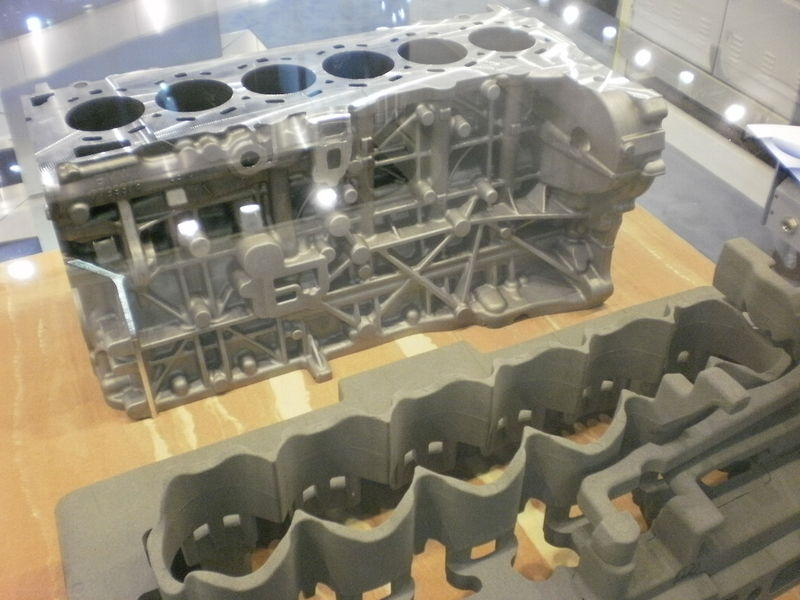
\includegraphics[height=2.5cm]{png/moteur}
\textit{Noyau pour moulage de moteur -- Moule en sable \cite{moteur}}
\end{center}
\end{minipage} \hfill
\begin{minipage}[c]{.2\linewidth}
\begin{center}
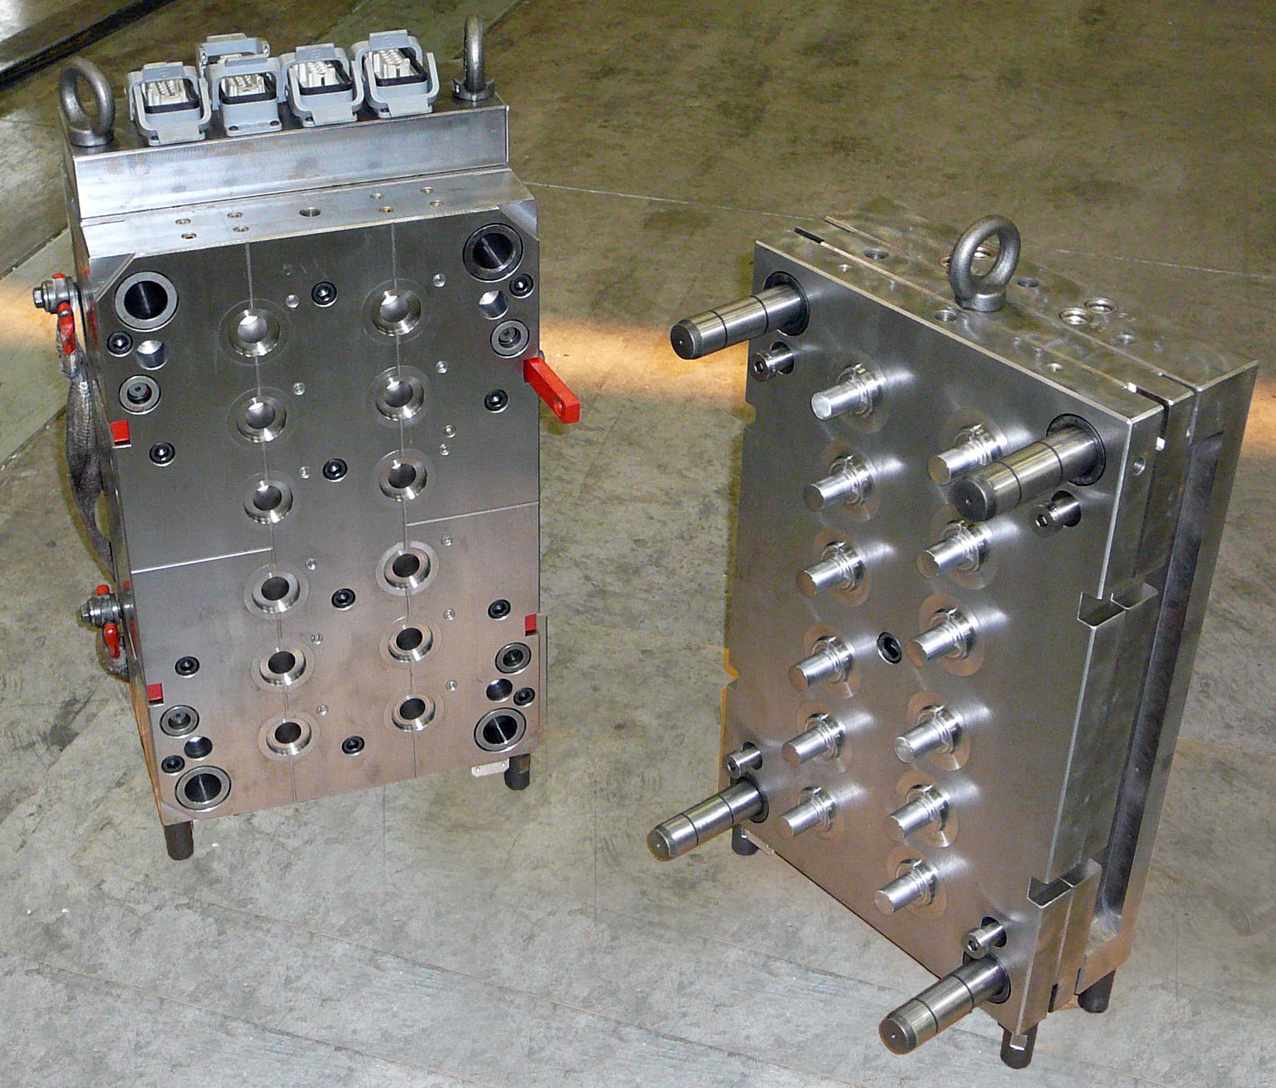
\includegraphics[height=2.5cm]{png/injection2}
\textit{Moules pour l'injection plastique \cite{injection}}
\end{center}
\end{minipage} \hfill
\begin{minipage}[c]{.2\linewidth}
\begin{center}
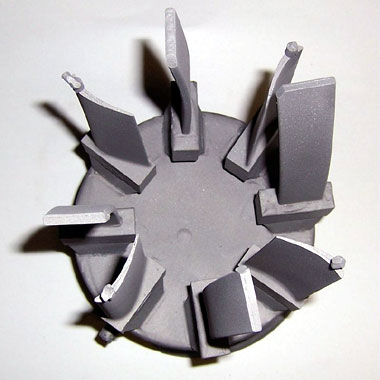
\includegraphics[height=2.5cm]{png/cireperdue}
\textit{Grappe d'aubes pour moulage à la cire perdue \cite{cireperdue}}
\end{center}
\end{minipage} \hfill
\begin{minipage}[c]{.2\linewidth}
\begin{center}
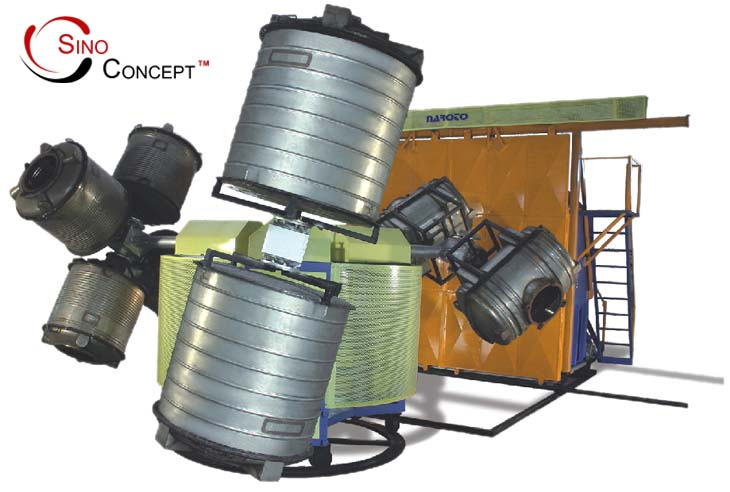
\includegraphics[width=.9\textwidth]{png/rotomoulage.png}
\textit{Machine de rotomoulage \cite{rotomoulage}}
\end{center}
\end{minipage}

\vspace{.5cm}





%\begin{center}
%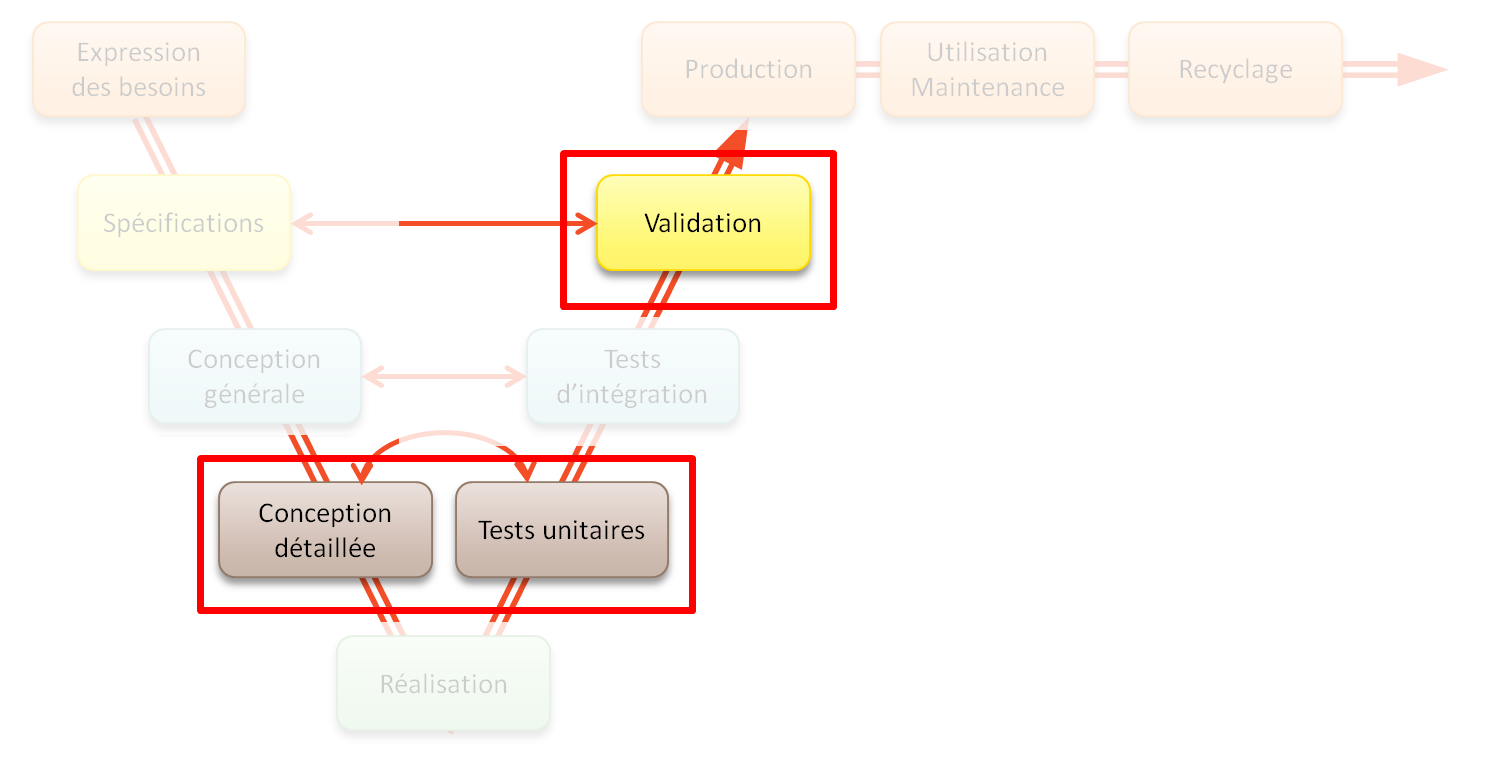
\includegraphics[width=.9\textwidth]{png/cyclev.png}

%\textit{Cycle de conception d'un produit}
%\end{center}

%\begin{prob}
%\textsc{Problématique :}

%En phase d'avant conception d'un produit, quels sont les critères qui vont permettre de choisir les matériaux à utiliser ?
%\end{prob}


Le fonderie est un procédé de mise en forme qui consiste à verser un matériau à l'état liquide dans un moule et à retirer ce matériau après solidification. La difficulté est alors de réaliser le moule.

Suivant la nature du matériau, la taille de la série, la géométrie de la pièce il existe plusieurs procédés de moulage :
\begin{itemize}
\item moulage au sable;
\item moulage en coquille;
\item moulage à la cire perdue;
\item injection plastique;
\item moulage RTM.
\end{itemize}

Le but de ce cours n'est pas de détailler tous ces procédés de moulages, mais de décrire en particulier le moulage au sable. Pour ce procédé, le moule est dit \textbf{destructible} et \textbf{le modèle non destructible}. Quelques généralités sur l'injection plastique seront introduites. 

\begin{savoir}
\textsc{Savoirs :}
\begin{itemize}
\item Connaître le procédé d'obtention des pièces moulées
\item Savoir concevoir une pièce moulée
\end{itemize}
\end{savoir}

%\newpage 

\setlength{\parskip}{0ex plus 0.2ex minus 0ex}
 \renewcommand{\contentsname}{}
 \renewcommand{\baselinestretch}{1}

\tableofcontents

 \renewcommand{\baselinestretch}{1.2}
\setlength{\parskip}{2ex plus 0.5ex minus 0.2ex}

% \vspace{1cm}
\textit{Ce document évolue. Merci de signaler toutes erreurs ou coquilles.}

%\newpage



\section{Obtention des pièces métalliques moulées en moule non permanent, à
modèle permanent}

\subsection{Applications de la fonderie}
\begin{minipage}[c]{.55\textwidth}
Contrairement au forgeage, la fonderie permet d'obtenir des pièces creuses à cavités complexes (culasses de moteur, bâtis de machine).

On peut obtenir des pièces de forme complexes qu'il suffira d'usiner
localement. L'approche de la forme définitive de la pièce permet un gain de
temps et de matière.
\end{minipage}\hfill
\begin{minipage}[c]{.4\textwidth}
\begin{center}
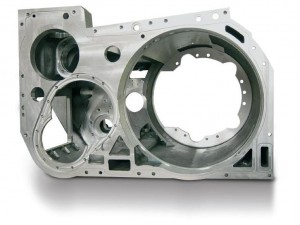
\includegraphics[width=.9\textwidth]{png/carter_moule}

\textit{Carter moulé de boîte de vitesse \cite{cartermoule}}
\end{center}
\end{minipage}

Il est possible de réaliser des pièces en matériaux difficilement usinables à
l'outil de coupe : 
\begin{itemize}
 \item ailettes de turbines ou de turbo réacteurs;
\item outils de coupe en acier rapide (fraise);
\item ...
\end{itemize}

Il est possible de réaliser des pièces en matériaux non malléables. 

Les alliages moulés ont les mêmes propriétés dans toutes les directions de
l'espace (isotropie). Le forgeage et le laminage ne permettent pas d'obtenir
cette propriété.

Les problèmes de moulage sont essentiellement des problèmes d'ordre géométrique.


\subsection{Description générale du procédé}
\begin{multicols}{2}
 
Ici, les moules sont détruits après la coulée. Ces moules sont généralement en
sable dont la cohésion est améliorée par addition d'argile, de ciment ou de
résine et par passage à l'étuve. 

Après avoir coulé le matériau en fusion et une fois la matière solidifiée, on
procède à la destruction de moule pour extraire la pièce. On réalise donc
autant d'empreintes (ou de moules) que de pièces à couler. 

\begin{center}
 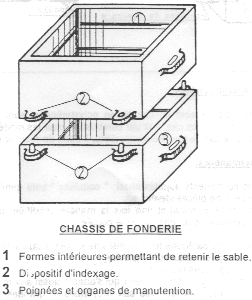
\includegraphics[width=.25\textwidth]{png/chassis}
\end{center}

\end{multicols}

Pour ce type de moule, l'empreinte s'obtient à partir d'un \textbf{modèle
permanent} que l'on imprime dans le sable et dont la forme correspond à celle
de la pièce à obtenir. 

Le moulage en moule non permanent à modèle permanent regroupe les technologie
de moulage au sable, de moulage en céramique, de moulage à la cire perdue. 

Ces procédés sont utilisés pour des pièces de moyennes à grandes dimensions et
pour des productions pouvant aller de l'unité jusqu'à la grande série. 

La fonderie en sable est cependant conditionnée par des problèmes de
manutentions du sable et des châssis. 

Pour illustrer le processus de fonderie au sable, prenons l'exemple de la
réalisation d'une bielle.

\begin{center}
\begin{tabular}{cc}
 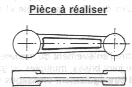
\includegraphics[width=.3\textwidth]{png/moulage1}&
 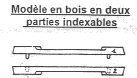
\includegraphics[width=.3\textwidth]{png/moulage2}
\end{tabular}
\end{center}


 
\begin{multicols}{2}
\begin{itemize}
 \item Mise en place sur la plaque «~porte modèle~» de la partie 1 du moule et
de l'attaque (3)
\item Apport du sable et tassage
\item Retournement de l'ensemble
\item Enlèvement de la plaque modèle
\end{itemize}

\begin{center}
 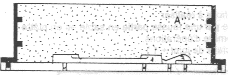
\includegraphics[width=.3\textwidth]{png/moulage3}
\end{center}
\end{multicols}


\begin{multicols}{2}
\begin{itemize}
 \item Mise en place du talc sur le plan de joint de A pour éviter le collage
avec le sable de B
\item Mise en place : 
\begin{itemize}
 \item du châssis supérieur
\item de la partie 2 du modèle
\item du mandrin de masselotte 5
\item du mandrin d'évent 6
\item du mandrin du trou de coulée 4
\end{itemize}
\item Apport du sable et tassage
\item Enlèvement de 4, 5, 6
\item Enlèvement et retournement de B
\item Enlèvement du modèle 1,2,3
\item Rectification de l'empreinte
\end{itemize}

\begin{center}
 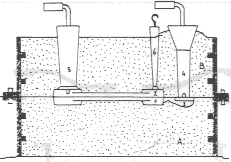
\includegraphics[width=.42\textwidth]{png/moulage4}
\end{center}
\end{multicols}

\begin{multicols}{2}
\begin{itemize}
 \item Remise de B sur A
\item Coulée
\item Refroidissement 
\item Effondrement du moule (marteau piqueur, chute libre, table vibrante)
\item Récupération de la pièce brute
\item Décochage
\item Ébarbage
\end{itemize}

\begin{center}
 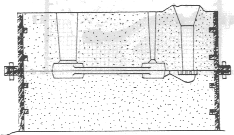
\includegraphics[width=.3\textwidth]{png/moulage5}
\end{center}
\end{multicols}

\begin{multicols}{2}
\begin{itemize}
 \item La masselotte est un appendice constituant une réserve de matière de
métal liquide capable d'alimenter les carences causées par la contraction du
métal au refroidissement dans la phase liquide + solide.
\item Évent : appendice permettant l'évacuation des gaz
\item Trou de de coulée : appendice vertical pour l'alimentation de l'empreinte
en métal liquide
\item Attaque : raccord entre le trou de coulée et l'empreinte.
\end{itemize}

\begin{center}
 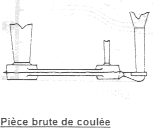
\includegraphics[width=.3\textwidth]{png/moulage6}
\end{center}
\end{multicols}

Remarques : 
\begin{itemize}
\item Pour pouvoir retirer le modèle du moule, il faut que les surfaces du
modèle perpendiculaire au plan de joint soient en dépouille pour ne pas
entraîner des particules de sable, le modèle et donc la pièce seront donc
légèrement coniques.
\textbf{L'angle de dépouille est de l'ordre de 2 à 3 degrés.}
\item Il faut faire un choix judicieux du plan de joint pour permettre
l'enlèvement du modèle. La forme de certaines pièces peuvent conduire au choix
de plans de joint brisés, multiples ou gauches. Ces problèmes sont traités par
le mouleur mais ils doivent également être envisagés par le bureau d'étude lors
de la conception de la pièce :
\begin{itemize}
\item un plan de joint gauche ou brisé est plus difficile à réaliser (la plaque
porte modèle est remplacée par une fausse partie en sable ou en plâtre);
\item des plans de joint multiples multiplient le nombre d'opérations (nombre
de châssis = nombre de plans de joint +1).
\end{itemize}
\end{itemize}



\subsection{Matériaux}
\subsubsection{Matériaux utilisables en moulage en moule non permanent}
Ce procédé de moulage est utilisable pour des types différents de métaux :
\begin{itemize}
 \item fontes lamellaires et malléables;
\item aciers; 
\item aluminium et alliages;
\item cuivre et alliages;  
\item alliages divers.
\end{itemize}


Du fait de l'utilisation de moules en sable, les métaux ayant une haute
température de fusion seront moulables en moules non permanents.



\subsection{Réalisation des formes extérieures}

\subsubsection{Matériaux constituants les moules destructibles}
Il existe une grande multitude de sables utilisables dans le cadre du moulage. 
Les sables sont choisis en fonction :
\begin{itemize}
 \item de leur prix de revient;
 \item de leur aptitude à être recyclée;
 \item de leur tenue à la température, à la pression;
 \item de la taille des pièces;
 \item du matériau moulé...
\end{itemize}

On distingue par exemple : 
\begin{itemize}
 \item le sable à vert : caractéristiques détaillées ci-après;
\item le sable à vert séché grillé flambé : accroissement de la dureté du sable;
\item le sable à vert étuvé : moule rigide sans humidité;
\item les sables agglomérés : la plupart sont utilisés pour réaliser les noyaux. 
\end{itemize}

Pour les moules destructibles, le sable est justement utilisé pour son aptitude
à être détruit pour démouler la pièce. Il a de plus la faculté de ne pas
changer d'état pour des hautes températures (supérieures à $1500^oC$). Il
résiste donc à la température lors de la coulée de la pièce.

\subsubsection{Moulage et organes de coulée}
Le moule doit comporter au moins deux parties (quelquefois plus) pou permettre
l'extraction du modèle. 

Chaque partie est enfermée dans un châssis. Il s'agit d'une caisse métallique,
sans fond, démontable, et dont les formes intérieures permettent de retenir le
sable. 

Le plan de jonction de deux châssis est appelé plan de joint. Lorsque deux
châssis sont superposés, ils sont \textbf{indexés} l'un par rapport à l'autre.



(moule, descente de coulée,
chenaux d’alimentation, masselotage, refroidissement)

\subsubsection{Procédé d'obtention du modèle}
Les modèles sont généralement réalisés en bois. Ils sont donc réalisés
manuellement par des menuisiers ou ébénistes spécialisés.

\subsection{Réalisation des formes intérieures}

\subsubsection{Matériaux utilisés pour les noyaux}
Les noyaux sont réalisés en sables agglomérés. On distingue parmi eux :
\begin{itemize}
 \item le sable à l'huile;
\item le sable aux résines thermodurcissables : employé pour le noyautage en
grande série. Le sable enrobé de résines est soufflé dans une boîte à noyau
métallique chauffée à $180^oC$. Durcissement en 10 secondes environ;
\item sable aggloméra aux résines à prise à froid grâce au procédé du silicate
de soude. Le durcissement est obtenu en quelques secondes par injection dans le
sable de gaz carbonique;
\item \textit{etc}.
\end{itemize}

\subsubsection{Procédé d'obtention du noyau}
Les noyaux sont obtenus par agglomération de sable. Ils sont généralement
agglomérés dans des «moules» appelées boîte à noyau. Suivant le type de sable
utilisé, le procédé de fabrication peut différer. 

\begin{center}
 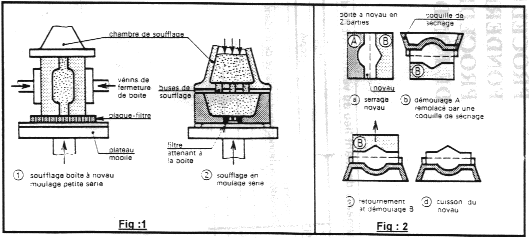
\includegraphics[width=.8\textwidth]{png/boite1}
\end{center}

\begin{center}
 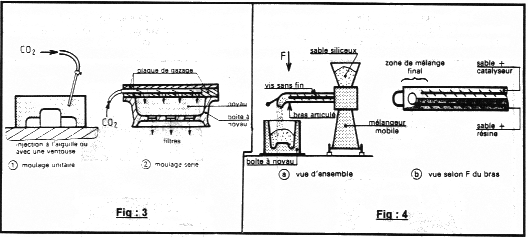
\includegraphics[width=.8\textwidth]{png/boite2}
\end{center}

\subsubsection{Dessin de noyau et portées associées}
Un noyau est une partie du moule très sollicitée (choc thermique à l'arrivée du
métal, choc mécanique, poussée d'Archimède ...)

Lorsque les dimensions des noyaux sont importantes, on réalise une armature
interne métallique qui, en plus d'augmenter la résistance, favorise leur
extraction dans les cavités complexes. 

Lorsqu'ils sont en porte-à-faux on peut les suspendre ou les déposer sur des
supports métalliques destinés à se dissoudre dans le métal en fusion. 

Ces dispositions doivent être évitées dans la mesure du possible par un tracé
judicieux de la pièce.

\begin{center}
 \rotatebox{90}{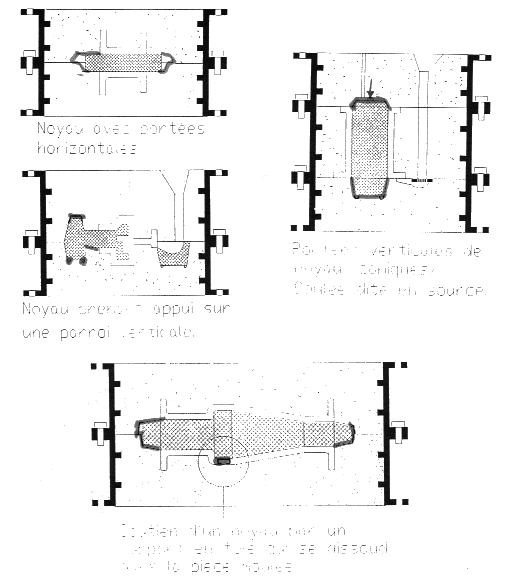
\includegraphics[height=.65\textwidth]{png/noyau1}}
\end{center}

\begin{center}
 \rotatebox{90}{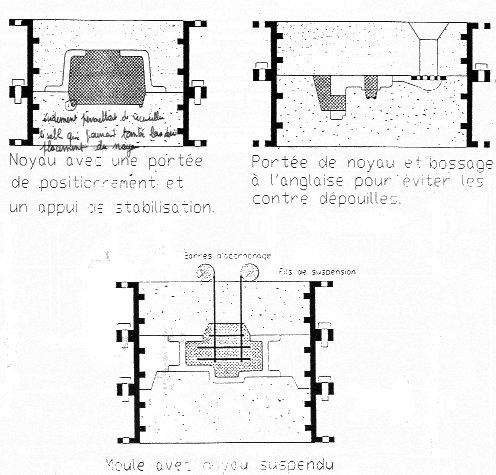
\includegraphics[height=.65\textwidth]{png/noyau2}}
\end{center}

\section{Conception des pièces moulées}


\subsection{Généralités}
3 principaux acteurs interviennent dans le déroulement de la fabrication d'une
pièce moulée : 
\begin{itemize}
 \item le concepteur : il définit parfaitement les exigences fonctionnelles et
les caractéristiques mécaniques de la pièce;
\item le préparateur : il organise le travail de réalisation, il a la charge de
la fabrication du produit, il prévoir les outillages, il minimise les usinages,
il définit ainsi un \textbf{brut minimal de fonderie};
\item le fondeur : il a la charge d'élaborer la pièce coulée en respectant les
exigences citées antérieurement, qui conditionnent la solution envisagée et
donc le prix de revient de la pièce à fabriquer. 
\end{itemize}

Idéalement, la solution serait d'obtenir directement la pièce la plus
économique possible avec le déroulement concepteur, préparateur, fondeur sans
concertation pour obtenir les délais les plus courts. Évidemment, cette
solution n'existe pratiquement pas et des concertations sont nécessaires pour
parvenir à la solution la plus intéressante.

Lors de la conception, le concepteur doit tenir compte des exigences de
fabrication de la pièce pour obtenir la solution la plus économique. 

Pendant toutes les phases de fabrication d'une pièce moulée (moulage, coulée,
refroidissement, démoulage, décochage...) un certain nombre de phénomènes
physiques sont mis en jeu. Ces phénomènes également appelés «facteurs de
fonderie», sont très nombreux et dépendent souvent les uns des autres. Ils
conditionnent la bonne qualité de la pièce moulée. 

Ces facteurs de fonderie sont relatifs: 
\begin{itemize}
 \item à la nature du métal ou des alliages et à ses propres propriétés
physiques : conductivité thermique, coefficient de dilatation, ségrégation;
\item aux conditions de fusion : température de chauffe et de fusion,
atmosphère dans le cubilot...; 
\item aux conditions de coulée : température de coulée, débit, pression ...;
\item au moule : forme, matériau, conditionnement, température...;
\item à la forme et aux dimensions de la pièce à fabriquer.
\end{itemize}

Le concepteur est concerné par le tracé des pièces moulées. Il doit en effet :
\begin{itemize}
 \item éviter les défauts dus à certaines propriétés physiques du métal;
\item éviter les défaillances des moules, des noyaux, des modèles;
\item simplifier ou minimiser toutes les opérations de moulage de la pièce.
\end{itemize}

Analysons les différents défauts de fonderie pour en tirer des règles générales
afin que le concepteur puisse réaliser le tracé le plus performant possible de
la pièce moulée. 

On peut diviser ces règles en trois groupes : 
\begin{itemize}
 \item les lois techniques de moulage avant et après la coulée : simplifier et
minimiser les opérations de moulage, les rendre les plus faciles et plus
fiables etc.;
\item les lois physiques de formation pendant la coulée et la solidification :
fusion, écoulement, coulabilité, retrait, hétérogénéité;
\item les lois de fonctionnement de la pièce : condition de résistance. 
\end{itemize}

Ces problèmes sont parfois antagonistes, le constructeur en tiendra compte en
fonction de la réalisation spécifique le concernant.

\subsubsection{Lois techniques de moulage avant et après la coulée}


Le but est de faciliter toutes les opérations et de minimiser leur nombre. 

\subsubsection*{Avant la coulée}

\paragraph*{Faciliter le moulage au niveau du moule, des noyaux et des modèles,
afin de diminuer le nombre de châssis et d'opérations.} 
\begin{center}
 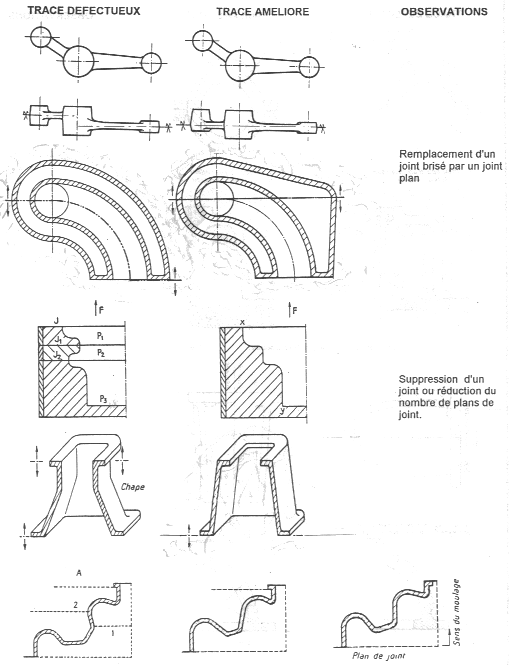
\includegraphics[width=.8\textwidth]{png/regles_plan}
\end{center}

\paragraph*{Adopter des formes de pièces se démoulant sans artifice suivant une
direction perpendiculaire au plan de joint, afin de faciliter le démoulage du
modèle.}
\begin{center}
 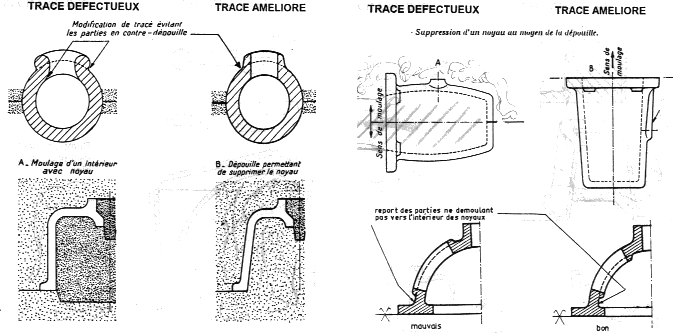
\includegraphics[width=.9\textwidth]{png/regles_depouilles}
\end{center}

\paragraph*{Rechercher des formes symétriques de pièces, afin de ne fabriquer
qu'une partie du modèle ou des boîtes à noyaux.}


\paragraph*{Rechercher des formes de pièces réalisées avec un nombre d'éléments
géométriques simples, afin d'assurer une précision dimensionnelle de forme et
de position améliorée.}

\paragraph*{Limiter le nombre de noyaux. En effet, le sable à noyau est plus
coûteux que celui de l'empreinte. De plus, la réalisation des noyaux nécessite
plus d'opérations.}

\begin{center}
 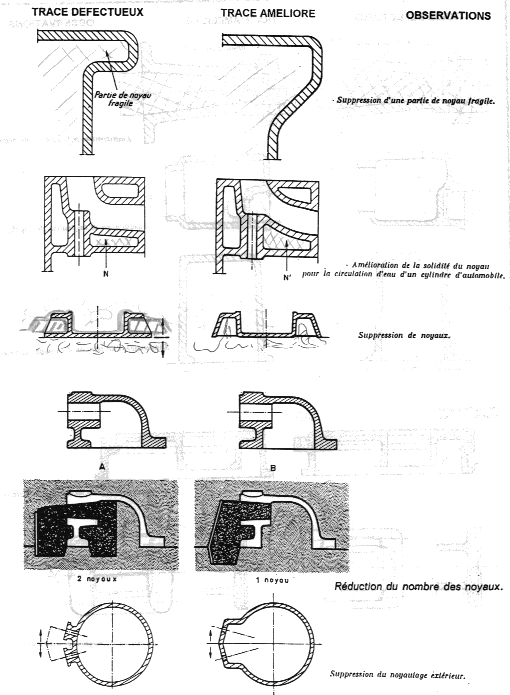
\includegraphics[width=.8\textwidth]{png/regles_noyau}
\end{center}

\paragraph*{Prévoir un positionnement facile, stable et précis des noyaux dans
le moule, afin de penser au remoulage avec des noyaux dans l'empreinte
inférieure.}

\begin{center}
 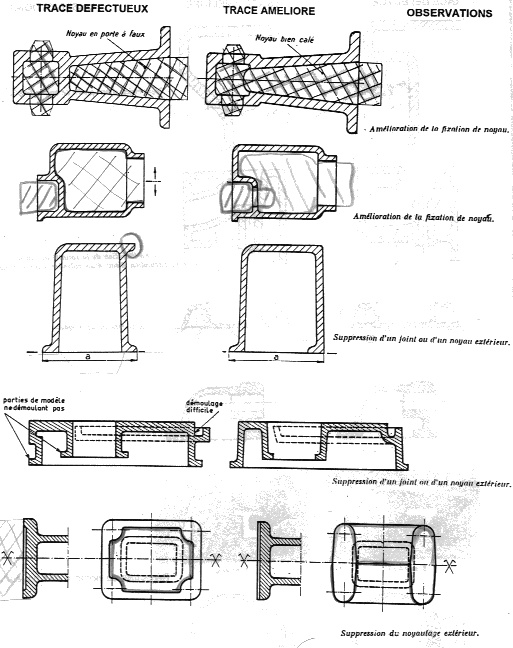
\includegraphics[width=.8\textwidth]{png/regles_noyau_2}
\end{center}

\paragraph*{Éviter la destruction de certaines parties fragiles des noyaux et
des empreintes, afin de dessiner des formes de pièces conférant une certaine
robustesse et rigidité des noyaux et empreintes. La durée de vie est améliorée.}


Pour un moulage en sable, les noyaux sont plus simples à mouler que les
empreintes. Il est donc préférable de reporter les difficultés de
moulage sur le noyau.

Pour un moulage en coquille, les formes intérieures doivent se démouler
normalement. Il est donc préférable de reporter les difficultés de
moulage sur les formes extérieures de l'empreinte. 


\subsubsection*{Après la coulée} 


\paragraph*{Faciliter le désablage, l'ébarbage, l'usinage.}

\begin{center}
 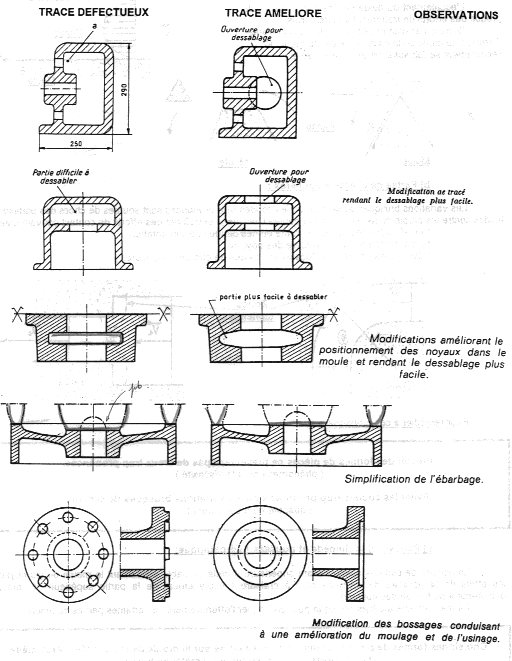
\includegraphics[width=.8\textwidth]{png/regles_ebarbage}
\end{center}

\paragraph*{Rechercher des formes extérieures qui ne retiennent pas le sable
après le décochage.}

\paragraph*{Prévoir des ouvertures suffisantes pour désablage et nettoyage des
formes intérieures de la pièce.}

\paragraph*{Faire coïncider si possible le plan de joint avec une surface de la
pièce, afin de rendre l'ébarbage plus facile et les décalages des moules moins
visibles.}

\paragraph*{Mettre dans un même plan si possible les surfaces devant être
usinées.}


% cahier des charges
% Agencement des zones fonctionnelles et des surfaces limites en fonction du
% cahier des charges
% démarche de tracé et adaptation des formes en fonction des sollicitations et
% de
% la faisabilité de moulage.
% 
% caractéristiques des pièces obtenues;

% \begin{itemize}
% \item d’identifier un plan de joint possible;
% \item de décrire les éléments caractéristiques de la pièce (dépouilles,
% nervures, congés, bossages, parois, défauts);
% \item de proposer les aménagements éventuels conduisant à des simplifications
% de
% la réalisation de la pièce.
% \end{itemize}
% 
% À partir du cahier des charges d'une solution technique, l'étudiant doit être
% capable :
% \begin{itemize}
%  \item de tracer les formes de la pièce en respectant les règles élémentaires;
% \item de tracer des pièces aux épaisseurs minimales;
% \item d'élaborer un dessin d'avant projet de la solution en proposant des
% dispositions de parois et des formes compatibles avec le procédé et le
% comportement de la pièce durant son cycle de vie.
% \end{itemize}
% 
% 
% On insiste sur le tracé des pièces moulées en présentant des études de cas.


\section{Phénomènes physiques mis en jeux lors du coulage des pièces}
\subsection{Écoulement du métal en fusion}
\subsubsection{Effets de la viscosité sur les parois du moule}
L'écoulement de fluide sur les parois du moule produit des efforts de
frottement liquide/parois.

Dans le cas d'un moule en sable, ceci entraîne l'érosion du canal ou la cassure
locale du moule si l'écoulement se fait autour d'une partie fragile. 

\subsubsection{Perte de charges singulières}
Les variations brusques de section ou les coudes trop prononcés sont sources de
chocs des particules fluides contre les parois du moule lors de la coulée. Ces
chocs entraînent des efforts de contact pouvant créer : 
\begin{itemize}
 \item un effondrement local du moule ou des conduits d'alimentation;
\item un déboîtement ou la rupture des noyaux;
\item des chutes de pression localisées (pertes de charges singulières).
\end{itemize}

Pour remédier à ces problèmes : 
\begin{itemize}
 \item prévoir des formes de pièces ne présentant pas de creux trop prononcés
(phénomène dû à la viscosité);
\item éviter les coudes trop prononcés où les variations brusques de section
(quantité de mouvement).
\end{itemize}

\subsubsection{Poussée d'Archimède et poussée hydrostatique}
La densité de certains alliages étant supérieure à celle du sable constituant
le moule ou les noyaux, les effets de la poussée d'Archimède sont à craindre
(soulèvement de la partie supérieure du moule, déboîtement ou flexion des
noyaux).

La pression latérale hydrostatique peut provoquer l'effondrement de certaines
parties du moule. 

Choisir des formes de pièces qui minimisent les effets sur le moule de la
poussée d'Archimède et de la pression hydrostatique du métal en fusion.

\begin{center}
 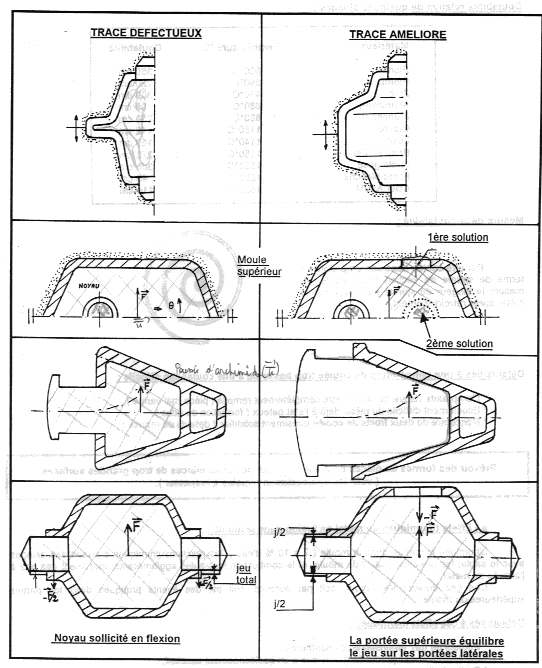
\includegraphics[width=.8\textwidth]{png/regles_physiques}
\end{center}
\subsubsection{Remplissage de l'empreinte : la coulabilité}
C'est l'aptitude du métal en fusion à remplir les cavités de l'empreinte. 

La coulabilité est liée à la viscosité du métal qui, elle même, dépend de la
température. 

Lorsque le métal avance dans le moule, il se refroidit au contact des parois,
sa viscosité augmente jusqu'au moment où sa propagation dans l'empreinte est
stoppée par les forces de viscosité (formation d'un bouchon). 

La coulabilité dépend donc de la température de coulée et de la nature du métal
ou de l'alliage (conductivité thermique, viscosité).

\paragraph*{Mesure de la coulabilité}
Par une coulée dans l'empreinte en forme de spirale de section trapézoïdale, on
mesure la longueur de spirale parcourue par le métal après refroidissement. 

\paragraph*{Coulabilité relative de quelques alliages}
\begin{center}
 \begin{tabular}{ccc}
  \hline
    Matériaux & Température & Coulabilité \\
\hline
Plomb         & $800^oC$  & $360\;cm$ \\
Plomb         & $390^oC$  & $220\;cm$ \\
Zinc          & $480^oC$  & $300\;cm$ \\
Aluminium     & $680^oC$  & $ 90\;cm$ \\
Aluminium     & $880^oC$  & $250\;cm$ \\
Cuivre        & $1150^oC$ & $172\;cm$ \\
Laiton        & $1140^oC$ & $189\;cm$ \\
Bronze (16\%) & $1150^oC$ & $276\;cm$ \\
Fonte grise   & $1300^oC$ & $300\;cm$ \\
Fonte blanche & $1250^oC$ & $ 43\;cm$ \\
\hline
 \end{tabular}
\end{center}

\paragraph*{Défauts liés à une température de coulée trop basse ou à une
coulabilité difficile}
\begin{itemize}
 \item L'empreinte risque de ne pas être complètement remplie (pièce mal venue).
\item L'écoulement difficile du métal déjà à l'état pâteux (formation de rides).
\item La rencontre des deux fronts de coulée quasiment solidifiés (défauts de
reprise).
\end{itemize}

Il faut donc prévoir des formes de pièces ne présentant pas de parois minces de
trop grandes surfaces (voir les épaisseurs minimales à respecter).

\subsubsection{Effets thermiques du métal en fusion dans le moule}
L'humidité contenue dans le moule (7 à 10\%  d'eau), les réactions chimiques à
chaud des alliages avec le sable avec les produits volatils du moule, et la
combustion locale des agglomérats produisent les gaz à l'arrivée du métal. 

Ces gaz doivent s'échapper soit par porosité, soit par des évents pratiqués
dans les parties du moule. 

Défauts liés à ces effets thermiques : 
\begin{itemize}
 \item poches de gaz emprisonnées (soufflures);
\item détérioration des parois du moule due à un bouillonnement excessif;
\item partie de l'empreinte non remplie par suite d'une importante poche de gaz
n'ayant pu s'évacuer, c'est un «refus» prévoir des évents. 
\end{itemize}


\textbf{Prévoir des formes de pièces permettant l'élimination naturelle des gaz,
des grains de sable et des impuretés (par gravité, par courant).}

\subsection{La solidification}

\subsubsection*{Le retrait}
Le métal se contracte pendant son refroidissement lorsqu'il se trouve sous ses
trois phases : liquide, liquide+solide, solide.

C'est pendant la phase intermédiaire que le retrait est le plus important. 

Les échanges de chaleur se font avec les parois du moule. Le gradient de
température est donc perpendiculaire aux surfaces de l'empreinte en leur
voisinage. 

Les isothermes orthogonales au gradient thermique sont donc quasiment
parallèles aux parois du moule sauf au niveau des angles où le flux thermique
dépend de la valeur de ceux-ci.

\begin{center}
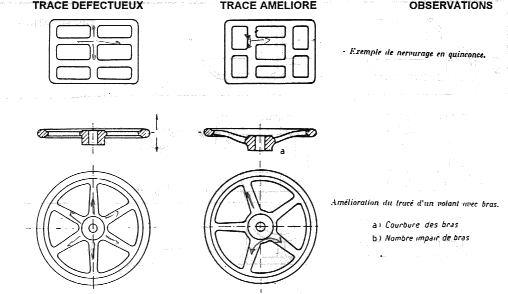
\includegraphics[width=.8\textwidth]{png/regles_retrait}
\end{center}


\paragraph*{Étude du refroidissement}
Le métal se contracte par abaissement de la température. Les parties froides
créent un appel de métal pendant la solidification. On observe un flux de métal
liquide à travers les surfaces isothermes. Ce métal liquide provient de la
partie centrale, plus chaude et se dirige vers les parties externes plus
froides. On assiste donc à la formation d'une cavité dans la partie supérieure
du lingot appelé \textbf{retassure}. Le retrait peut être réduit en abaissant
la température de coulée mais, dans ce cas, la coulabilité diminue. 

Le même phénomène de produit pendant la phase de solidification, si une partie
massive du métal se solidifie sans être alimentée en permanence en liquide, il
se produit une \textbf{retassure interne}. 

La masselotte est un appendice de la pièce moulée, enlevé après démoulage. Son
but est de nourrir en métal liquide les parties qui se solidifient en dernier.
Les masselottes peuvent également servir de trou de coulée ou d'évent
(évacuation des gaz et des impuretés). Elles peuvent être internes ou externes. 

Lorsque la partie massive isolée n'est pas très importante, on observe une
multitude de retassures microscopiques que l'on appelle \textbf{porosités}. 

Si on peut traiter le problème à la conception de la pièce, le mouleur peut y
remédier par des masselottes ou des refroidisseurs. 


\paragraph*{Pour éviter les retassures et les porosités}
Éviter les parties massives isolées.


\begin{center}
 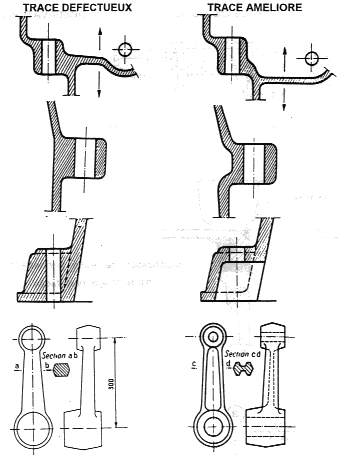
\includegraphics[width=.6\textwidth]{png/regles_massive}
\end{center}

Respecter les règles de raccordement des parois. 

\begin{center}
 \rotatebox{90}{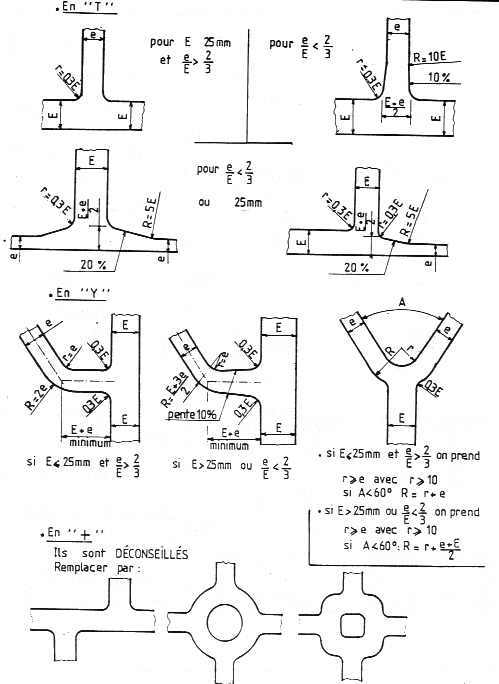
\includegraphics[height=.85\textwidth]{png/regles_raccord1}}
\end{center}

\begin{center}
 \rotatebox{90}{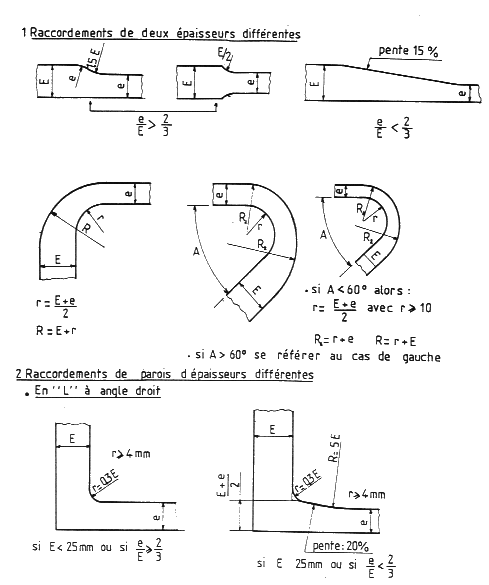
\includegraphics[height=.85\textwidth]{png/regles_raccord2}}
\end{center}


Donner les formes permettant une alimentation naturelle en métal liquide
(prévoir une solidification dirigée). 

Épaisseurs constantes et progressives. Pas d'angles vifs.

\paragraph*{Solidification dirigée}
Le moule étant rempli, le front de solidification progresse depuis les parties
les moins épaisses et se dirige vers les plus épaisses. Le courant de métal qui
alimente les zones de solidification est l'inverse du sens de déplacement du
front ci-dessus.

Pour éviter la formation du bouchon, il faut une augmentation progressive de
l'épaisseur de la pièce, la partie la plus massive étant reliée à une
masselotte permettant de compenser les carences en métal liquide causées par le
retrait.



\subsubsection{Retrait phase solide}
\paragraph*{Retrait à haute température}
Lorsque le rayon de raccordement de deux parois est trop petit, la résistance à
chaud du métal solidifié au voisinage de cet arrondi n'est pas suffisante à
cause de la mauvaise évacuation de la chaleur, il se produit alors une crique. 

Exemple : 
\begin{itemize}
 \item mauvaise évacuation de la chaleur en A
\item isothermes serrées, la résistance à chaud du métal est inférieure dans la
zone entourée. 
\item rupture sous les efforts de F et F' engendrés par le retrait, formation
d'une crique.
\end{itemize}

Respecter les règles de raccordement citées précédemment, ces derniers tiennent
compte du flux thermique au voisinage des arrondis intérieurs et évitent en
général la formation de criques (les isothermes sont à peu près parallèles).


Étudier la forme de la pièce de manière à ce que les forces engendrées par le
retrait à haute température en phase solide ne sollicitent pas une zone trop
faible de la pièce.

\subsection{Lois de la résistance des matériaux}
Les lois de la résistance des matériaux permettent au concepteur de déterminer
les formes et les dimensions de la pièce nécessaires à un bon fonctionnement de
celle-ci. 

Exemple : il faut veiller à ce que les sections les plus fortes soient
sollicitées en traction et les sections les plus minces en compression.

\begin{center}
 {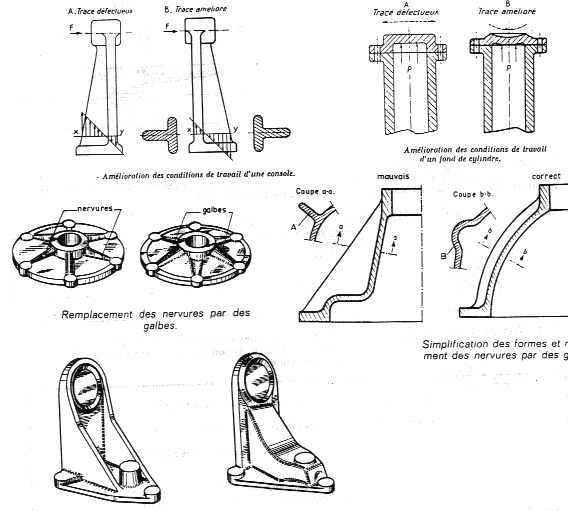
\includegraphics[height=.7\textwidth]{png/regles_resistance}}
\end{center}

\section{L'injection plastique}
\textit{Vous trouverez ici des informations sur l'injection plastique. Ces
informations sont données à titre indicatif.}

       L'injection des polymères permet d'obtenir en une seule opération des
 pièces finies, de  formes  complexes,  dans  une  gamme  de  poids  de 
quelques  grammes  à plusieurs  kilogrammes. 
\begin{multicols}{2}

\begin{center}
 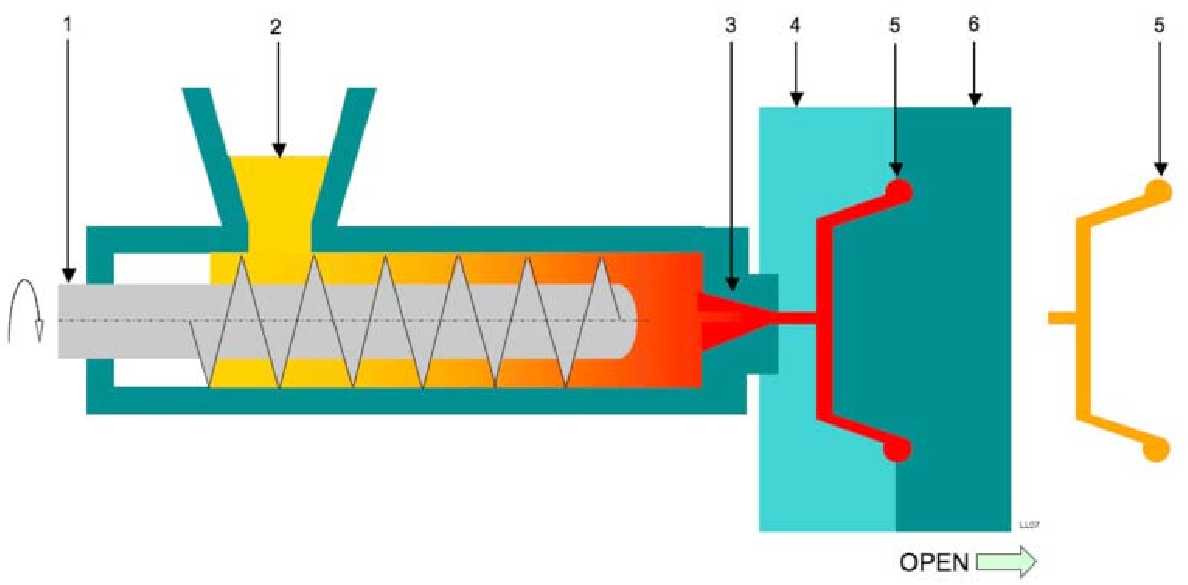
\includegraphics[width=.45\textwidth]{png/injection}
\end{center}
                                
\begin{enumerate}
\item Vis de plastification contrôlée par la presse     
\item Trémie d'alimentation 
\item Buse d'injection 
\item Partie fixe du moule 
\item Empreinte/pièce 
\item Partie Mobile du moule
\end{enumerate}

       1+2+3 = Cylindre de plastification                                   
    
       
\end{multicols}
        Les  fonctions  du  système  de  plastification  et  d'injection 
consistent  à  fondre  la  matière plastique et à l'injecter dans le moule. 

        La presse est là pour contrôler la vitesse et la pression d'injection de
la matière dans le moule. 

        Contrairement  au  moulage  de  pièces  métalliques,  le  temps  de 
cycle  pour  fabriquer  une  pièce  en  injection,  dépasse  rarement  la 
minute,  de  plus  le  moule est  constamment régulé par un circuit de
refroidissement. 

Tout  d'abord,  l'empreinte  du  moule  est  remplie  en  moins  d'une 
seconde  pour  les petites  pièces  (touches  de  téléphones 
portables,  presse étoupe...)  et  en  quelques secondes  pour  les 
pièces  de  plus  gros  volumes  (dossier  de chaise,  pare-chocs  de  
voiture, pièces de carrosserie...). 

Ensuite vient la phase de maintien ou de compactage durant laquelle la
presse met l'empreinte sous pression en injectant plus de matières afin
de combler le retrait du plastique. 

Pour finir les pièces sont extraies par un kit d'éjection. 

        \subsection{L'outillage}

     
\begin{multicols}{2}
 
\begin{center}
 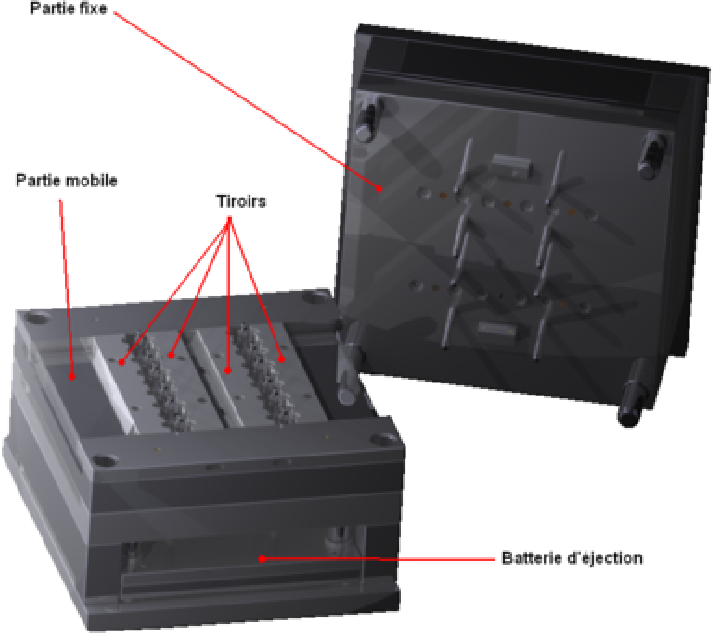
\includegraphics[width=.35\textwidth]{png/moule_inject}

Moule à 4 tiroirs 
\end{center}


    L'outillage ou moule, est en général constitué d'une partie fixe fixée sur
la presse, d'une  partie  mobile  qui  va  se  déplacer  pour  pouvoir  libérer 
la  pièce  une fois  refroidie  et  d'un 
système d'éjection chargé de pousser la pièce en dehors du moule. 

Un  moule,  doit remplir  plusieurs fonctions : 
\begin{itemize}
 \item fonction mise en forme 
\item fonction alimentation 
\item fonction régulation 
\item fonction refroidissement de la pièce 
\item fonction éjection 
\end{itemize}
\end{multicols} 
 
           
        \subsubsection{Fonction mise en forme ou empreinte}
        Dans un moule d'injection le nombre d'empreintes est généralement un
nombre pair 
(en  dehors  des  moules  mono  empreinte)  ceci  est  fait  pour  des  raisons 
d'équilibrage  de 
remplissage. 
        Le choix du nombre dépend essentiellement de la quantité à produire à
fin de vie du 
moule. 
        
        La forme de la pièce se fait par l'empreinte qui se répartit entre les
deux parties (fixe 
et  mobile)  du  moule  et  d'autres  éléments  auxiliaires  tel  que  (tiroirs 
-cales  montantes-
noyaux)  dans  le  but  de  faire  des  formes  en  contre  dépouilles  (des 
formes  qui  ne  se 
démoulent pas dans le même axe d'ouverture du moule) 
        
\subsubsection{Fonction alimentation}

       La fonction alimentation a pour but de transférer la matière plastifiée
du fourreau de 
la presse, vers l'empreinte du moule. Au cours de ce cheminement, la matière est
soumise à 
différentes contraintes en passant par : 
\begin{itemize}
\item La buse d'injection, 
\item Le reçu de buse du moule 
\item Les canaux d'alimentations 
\item Les points d'injection 
\item Les formes de la pièce 
\end{itemize}

        Il existe deux grands types de canaux d'alimentation : 
\begin{itemize}
 \item Les canaux d'alimentations standards : Ils sont placés directement dans
la plaque du moule et doivent être démoulés comme la pièce après chaque
injection. La matière utilisée pour les canaux à chaque injection est perdue. 
\item Alimentation sans déchets ou canaux chauds : Ils doivent conduire la
matière moulée dans  l'empreinte  sans  déperdition  de  chaleur.  Ils 
sont  chauffés séparément  de l'outillage (entre $180^oC$ et $300^oC$
suivant la matière injectée).
Techniquement il faut donc  isoler  le  canal  du  reste  de 
l'outillage  dont  la 
température  est  nettement inférieure. La matière du canal n'est pas perdue. 
\end{itemize}


        \subsubsection{Fonction régulation}
        La régulation de la température de l'outillage se fait à travers un
liquide caloporteur 
qui peut être: 
\begin{enumerate}
 \item l'eau pour des températures faibles (eau à $15^oC$) 
\item l'huile pour des températures allant à $130^oC$ 
\end{enumerate}

        
        Ce liquide est envoyé à travers des canaux percés dans la carcasse de
l'outillage et les 
empreintes en utilisant un thermorégulateur. 

        \subsubsection{Fonction éjection}

        La plupart des pièces réalisées par injection plastique resteraient dans
le moule après 
son ouverture et ne seraient pas évacuées sous l'effet de la gravité seule si
aucun système 
d'éjection n'existait. 
        Plusieurs  systèmes  ont  donc  été  conçus  afin  d'aider  l'extraction
 de  la  pièce  à 
l'ouverture du moule : 
         \paragraph{Les éjecteurs}
         Les  éjecteurs  sont  des  barres  métalliques  cylindriques  pleines 
(parfois  creuses)  qui, 
lors de l'ouverture du moule, viennent pousser la pièce plastique pour
l'extraire du moule. Il 
s'agit de la technique d'éjection la plus utilisée car elle peut s'appliquer à
quasiment toutes 
les  pièces  plastiques.  Les  traces  des  éjecteurs  sont  souvent  visibles 
sur  la  pièce  et  sont 
considérées  comme  "inesthétiques".  Les  concepteurs  de  pièces  injectées 
s'arrangent  alors 
pour que ces traces d'éjecteurs se situent sur la partie cachée de la pièce
plastique lors de 
son utilisation. 
         \paragraph{Les plaques dévêtisseuses}

         La fonction de la plaque dévêtisseuses est la même que celle des
éjecteurs. Il s'agit 
d'une plaque qui va venir pousser sur les bords d'une pièce. Ces bords doivent
donc se situer 
dans  un  même  plan.  L'avantage  principal  d'une  plaque  dévêtisseuses  est 
le  fait  qu'aucune 
marque n'est réellement visible sur la pièce finie. 
         \subsection{Conception des pièces injectées}
         La conception de pièces injectées est un métier qui consiste à adapter
une pièce afin 
de  faciliter  sa  fabrication  par  injection  plastique.  « L'art »  de 
concevoir  une  pièce  injectée 
consiste  à  concevoir  une  pièce  respectant  toutes  les  contraintes 
exigées  par  la  technique 
d'injection, tout en respectant le cahier des charges. 

\subsubsection{Les contraintes de conception}
         Des  règles  de  conception  pour  les  pièces  injectées  ont  été 
définies  grâce  à 
l'expérience  industrielle  dans  le  domaine  soit :l'éjection  de  l'air 
poussé  par  le  plastique 
pendant l'injection, la diffusion égale du plastique dans le moule, la position
des poussoirs 
qui éjecte la ou les pièce(s) finis, les pièces mobiles dans le moule, etc. 
         
\paragraph{Les dépouilles}
         Afin  de  faciliter  l'extraction  de  la  pièce  à  l'ouverture  du 
moule,  ou  afin  de  ne  pas 
arracher  de  la  matière lors  de  l'extraction  de  la  pièce,  aucune  face 
de  la  pièce  injectée  ne 
doit être strictement perpendiculaire au plan de joint du moule (autrement dit,
aucune face 
ne doit être strictement parallèle à la direction d'ouverture du moule). Si ce
n'est pas le cas, 
on  dit  de  cette  face  qu'elle  n'est  pas  dépouillée.  Exceptionnellement, 
et  pour  des  raisons 
fonctionnelles,  des  exceptions  peuvent  survenir  et  certaines  faces 
peuvent  ne  pas  être 
dépouillées. La surface de ses faces doit alors être la plus petite possible. 

         Afin  de  pouvoir  démouler  la  pièce,  aucune  face  ne  doit 
comporter  de  dépouille 
négative. Une dépouille positive minimum est souvent citée, valant 2 degrés. 

         Lors  de  dépouille  négative,  on  parle  alors  de  contre-dépouille.
 Celles-ci  ont  besoin 
d'un système adapté pour pouvoir permettre l'éjection de la pièce (cale-montante
ou tiroir). 

\paragraph{Les épaisseurs constantes}

         Pour  éviter  de  nombreux  défauts,  il  est  conseillé  d'avoir  des 
épaisseurs  constantes. 
Cela permet une bonne homogénéité de la matière et limite la présence de
retassures ou de 
vacuoles. 

        De  plus  en  injectant  des  pièces  d'épaisseurs  fines,  il  est 
possible  de  se  dispenser 
d'astuces telles que les masselottes qui sont difficiles à gérer (taille,
position, efficacité...) 

\paragraph{Le nervurage}

        Comme nous l'avons vu précédemment, il est conseillé d'avoir de fines
épaisseurs de 
pièces.  Malheureusement,  dans  certain  cas,  les  pièces  moulées  subissent 
des  contraintes 
importantes pouvant entraîner leurs ruptures. 
        Pour  pallier  ce  problème,  il  faut  renforcer  la  pièce  tout  en 
gardant  de  faibles 
épaisseurs. Le seul moyen à notre disposition est de mettre des nervures
(généralement un 
triangle rectangle isocèle d'épaisseur de la pièce). 
        La forme des nervures ne gène pas le moulage et démoulage (angle de
dépouille) et 
la pièce est renforcée 
 \subsection{Défauts des pièces injectées}
        \subsubsection{Retassures}
        Description : 
        Les retassures sont dans leur grosse majorité des défauts de surface
caractérisés par 
un affaissement de la matière, parmi elles: 

\begin{itemize}
 \item les  retassures  localisées :  au  voisinage  de  zones  avec  fortes 
variations  d’épaisseurs 
        (nervures) 
 \item les retassures en osselets : le retrait de matière s’effectue sur une
grande surface, de 
        façon à se décoller de la paroi par pellicules (sauf sur les bords).
\end{itemize}
 
         
        Mécanismes de formation : 
        Après le remplissage de l’empreinte, la matière chaude se rétracte (le
retrait dépend 
de la matrice polymère utilisée, et des charges présentes : PA6GF30 retrait de
0,1\% en sortie 
de  moule).  La  pression  de  maintien  appliquée  pour  compenser  ce  retrait
 ne  joue  pas  son 
rôle. 
        Causes possibles: 
\begin{itemize}
 \item la pression de maintien est insuffisante, ce qui rend possible un retrait
de la matière 
 \item la  vitesse  d’injection  est  trop  rapide,  ce  qui  rend  difficile 
le remplissage  et  rend ineffectif le maintien 
 \item le matière est déjà solidifiée au niveau du seuil ce qui entraîne des
difficultés pour le maintien 
 \item les paramètres choisis accentuent le retrait 
\end{itemize}

        Actions correctives : 
\begin{itemize}
 \item  renforcer la pression de maintien 
 \item  baisser  la  vitesse  d’injection et augmenter la température  de 
la matière  pour  faciliter  le remplissage. 
 \item  améliorer  la  conception  du  moule  (éviter  les  variations 
d’épaisseurs  des  pièces, placement du seuil d’injection) 
 \item  augmenter la température du moule et diminuer la température de la
matière (homogène) 
        
\end{itemize}
 
  
\subsubsection{Jet libre}
       Mécanismes de formation : 
       La  matière  sort  du  seuil  d’injection  à  la  façon  d’un  jet  d’eau
 à  la  sortie  d’un  tuyau d’arrosage.  Le  remplissage  de  l’empreinte  se 
fait  en  mode  turbulent, avec  une 
décompression brutale en sortie de seuil. 
        
       Causes possibles: 
\begin{itemize}
 \item mauvaise  conception  du  moule :  seuil  d’injection  mal  positionné 
(ou  mal dimensionné) 
 \item matière trop visqueuse 
 \item pression au niveau de seuil trop importante 
       Actions correctives : 
 \item améliorer la conception du moule ( augmenter la section du seuil) 
 \item augmenter la température de la matière 
 \item injection lente au début, puis plus rapide 
\end{itemize}
 
       \subsubsection{Défauts en ligne de soudure}
       Description : 
\begin{itemize}
 \item ligne de soudure marquée 
 \item mauvaise résistance mécanique des lignes de soudure 
 \item stries de couleur 
 \item forte retassure le long de la ligne de soudure 
       Mécanismes de formation : 
 \item apparaît en fin de remplissage, la surpression dépasse le pression de
maintien 
 \item la jonction est facilement cassable 
 \item dégradation de la coloration due à la température 
       Causes possibles : 
 \item mauvaise pression d’injection 
 \item température trop basse de la matière injectée 
 \item dégradation de la matière due à une surchauffe 
       Actions correctives : 
 \item augmenter la température de la matière 
 \item augmenter la vitesse d’injection 
 \item augmenter la température du moule 
 \item diminuer le trajet d’écoulement de la matière 
\end{itemize}
 
       \subsubsection{Cernes et sillons}
       Description: 
\begin{itemize}
 \item les  cernes,  ou  effet  fleur  sont  des  sillons  concentriques  mats 
autour  du  seuil d’injection. 
 \item les sillons, ou effets slick-slip sont concentriques et plus ou moins
creusés autour du seuil d’injection, ou dans les zones de faible
épaisseur. 
\end{itemize}
 
       
       Mécanisme de formation: 
       Le flux de matière pulse dans le moule, car il avance trop lentement. Le
défaut est en 
général plus courant dans les matières amorphes, plus visqueuses à chaud. 
        
       Causes possibles : 
\begin{itemize}
 \item mauvaise introduction de la matière injectée 
 \item mauvaise température de la matière 
 \item mauvaise conception du moule 
\end{itemize}
 
       Actions correctives :
\begin{itemize}
\item augmenter les vitesses d’injection 
 \item adapter les flux de matière (remplissage régulier) 
 \item augmenter la température de la matière 
 \item augmenter la température de l’outillage 
 \item augmenter l’épaisseur des pièces 
\end{itemize}
 
       \subsubsection{Entraînement d’air}
       Causes possible : 
       L’air inclus peut provenir : 
\begin{itemize}
 \item d’une mauvaise plastification lors du dosage 
 \item d’une mauvaise conception du moule ( aspérités, rayures,
renforcements...) 
\end{itemize}
 
       Action correctives : 
\begin{itemize}
 \item vérifier la qualité de la vis, choisir une unité de plastification
adapté au volume de la matière 
 \item augmenter la contre pression de la vis lors du dosage (freiner le recul
de la vis) 
 \item limiter la phase de décompression de la matière après dosage (diminuer
la course de décompression) 
 \item améliorer la conception du moule permettant l’évacuation de l’air 
 \item Utiliser un équipement de « sous-vide / vacuum » afin d'extraire l'air
/gaz présents dans le moule avant l'injection. 
\end{itemize}
 
       \subsubsection{Sous-dosage -- surdosage}
       Description des défauts engendrés et mécanisme de formation : 
                                                                    
\begin{itemize}
 \item en cas de sous-dosage le pièce obtenue est incomplète 
 \item pour un surdosage, l’excès de matière se traduira par des bavures
(pouvant boucher jusqu’aux  éjecteurs),  un  sur-compactage  (contraintes 
internes, cassures, déformations. 
\end{itemize}
       Causes possibles: 
\begin{itemize}
 \item quantité de matière injectée insuffisante ou trop importante 
 \item matelas de matière instable ou nul 
 \item clapet anti-retour de la vis de plastification usé ou cassé 
       Action correctives: 
 \item diminuer ou augmenter le dosage de matière 
 \item vérifier que le matelas de matière en fin d'injection est constant 
       
 \item changer le clapet anti-retour de la vis de plastification 
\end{itemize}
 \subsubsection{Bulles – effets fontaine}
         
        Mécanisme de formation: 
        Surtout  pour  les  pièces  de  forte  épaisseur,  le  remplissage  se 
fait  par  couches 
successives. La matière solidifiée en dernier se trouve à cœur, donc il peut y
avoir formation 
de bulles (et être assimilées à des retassures) 
         
        Action correctives: 
\begin{itemize}
 \item augmenter la vitesse d’injection 
\end{itemize}
 
        
% \subsubsection{Commutation précoce – commutation tardive}
%         Description de défauts engendrés par une commutation trop précoce : 
%         Il existe une série de défauts déjà traités: 
%  \item  pièce incomplète 
%  \item  présence de contraintes internes (cassures, déformations) 
%  \item  mauvaises lignes de soudure 
%  \item  écaillage  (matière  déjà  refroidi  déplacée  par  de  la  matière 
% chaude)  alternance  de 
%         zones mate et zones brillantes. 
%  \item  taches  mates  (matière  déjà  refroidi  déplacée  par  de  la 
% matière 
% chaude)  zone 
%         satinée/mate 
%  \item  défauts de cristallisation en forme de doigt (alternance de zones de
% refroidissement 
%         lente  et  rapide  dû  à  une  différence  de  cristallinité) 
% accentué 
% par  un  maintien  trop 
%         faible et une température du moule trop élevée. 
%         Actions correctives: 
%  \item  déplacer le point de commutation (passage de la phase injection à la
% phase maintien) 
% 
% \subsubsection{Conséquence d’une commutation décalée}
%         Une  commutation  tardive  est  assimilée  à  un  surdosage.  En  cas 
% de  commutation 
% précoce, on réalise un sous dosage compensé par la pression de maintien. Mais
% la
% matière 
% plus refroidie sera moins homogène. 

\subsubsection{Défauts dimensionnels}
        Actions correctives: 
        Pour des précisions dimensionnelles fines (micron), il faut: 
\begin{itemize}
 \item  une régulation en température précise du moule 
 \item  un moule très rigide 
 \item  éviter les contraintes internes 
 \item  une bonne prévision du retrait 
 \item  surface de l’empreinte de grande qualité (rayure, corrosion,
abrasion...
\end{itemize}

 
%         11.4.11 Matière humide avant transformation 
%         Description: 
%     
%          Selon la quantité d’humidité, le défaut à plusieurs aspects : 
%  \item   givrage (microbulles forment des stries blanches en touffes) 
%  \item   taches blanches (imperfection de surface ressemblant à de la
% moisissure) 
%  \item   petites bulles (bulles dans la matière, aspect mousseux) 
%          Mécanisme de formation: 
%          L’humidité présente dans la matière se transforme en vapeur d’eau
% lors
% du chauffage 
% dans le fourreau et s’évacue sous forme de bulles de gaz 
%           
%          Causes possibles: 
%          La matière transformée à absorbé l’humidité 
%           
%          Actions correctives: 
%          Etuver la matière avant transformation Mettre en place des trémies
% désicatrices 
%          Pour certaines matières plastiques, obtenues par polymérisation par
% condensation, la 
% reprise  d'humidité  avant  injection  peut  avoir  de  lourdes  conséquences 
% sur  les  propriétés 
% mécaniques de la pièce finie. En effet, sous l'effet de la chaleur, l'humidité
% présente dans la 
% matière va se transformer en vapeur d'eau. Celle ci va produire une réaction
% d'hydrolyse sur 
% les chaines macromoléculaire et briser certaines liaisons chimiques rendant
% ainsi le matériau 
% plus  fragile.  Ce  phénomène  est  facilement  observable  sur  les 
% polybutylènes  téréphtalates 
% (PBT) 
         \subsubsection{Incorporation d’éléments étranger – mauvais mélange}
         Description des défauts: 
\begin{itemize}
 \item délamination (perte de lamelles) ou exfolions (pellicules) 
 \item marbrures mauvaise homogénéisation des couleurs) 
 \item présence de corps métalliques : signe d’une détérioration de la
vis/outillages. 
\end{itemize}

        Causes possibles: 
\begin{itemize}
 \item alimentation matière polluée (poussière, métal) 
 \item outillage dégradé 
 \item mauvaise plastification 
\end{itemize}

         Actions correctives : 
\begin{itemize}
 \item   incorporer une grille magnétique à la trémie 
 \item   éviter les mélanges 
 \item   adapter les paramètres de plastification à la matière 
\end{itemize}

         
% \subsubsection{Combustion ou effet diesel - carbonisation}
%          Description 
%  \item   apparition de zones brûlées (aux extrémités) 
%  \item   coup de feu 
%  \item   strie de surchauffe 
%  \item   cratères (piqures, pustules) 
%  \item   écarts de couleur 
%  \item   dégradation des propriétés mécaniques 
%          
% 
%        Causes possibles : 
%        Des  bulles  de  gaz  sont  comprimées  et  s’enflamment  sous 
% l’effet 
% de  la  T°  (principe 
% moteur Diesel). 
%         
%        Action correctives : 
% \itemaméliorer la conception du moule 
% \itemoptimiser les paramètres (baisser vitesse d'injection, T° et pression) 
% \itemtempérature matière trop haute 
% \itemajouter des évents sur le moule 
% \itemUtilisation d'un équipement de « sous-vide / vacuum » ; en ôtant l'air /
% gaz présents 
%        dans le moule, on diminue considérablement le risque de « brûlures » 
       \subsection{Problèmes de démoulage}
       \subsubsection{Marquage des éjecteurs}
\begin{itemize}
\item Déformations 
\item Les éjecteurs transpercent la pièce au moment de l'éjection 
\end{itemize}

       Causes possibles : 
\begin{itemize}
 \item température matière trop importante au moment de l’éjection 
 \item pression interne trop élevée 
 \item mauvaise taille/disposition des éjecteurs 
\end{itemize}
       Actions correctives : 
\begin{itemize}
 \item augmenter le temps de refroidissement 
 \item adapter le profil des vitesses d’injection 
 \item adapter la vitesse des éjecteurs 
 \item baisser la température du moule 
 \item vérifier que les éjecteurs soit correctement montés 
\end{itemize}
       \subsubsection{La pièce reste coincée dans le moule – dégradation
mécanique de la pièce}

       Description: 
       Dégradations irréversibles : 
\begin{itemize}
 \item cassures 
 \item rainures 
 \item fissures 
\end{itemize}
       Causes possibles / correction: 
\begin{itemize}
 \item pression interne trop élevée 
 \item la pièce reste coincée sur ses parois externes : l’éjection est trop
précoce 
 \item la pièce reste coincée sur ses parois internes : l’éjection est trop
tardive
\end{itemize}

 
\subsubsection{Tirage de fil}
        
        Un long fil de matière sort de la buse jusque vers la carotte, ce qui
gêne l’éjection ( la 
carotte reste accrochée). 
         
        Causes possibles / correction: 
        La  matière  restée  dans  la  buse  au  moment  de  démoulage  est 
trop  chaude  ou  trop 
comprimée 
%         11.5 L'injection gaz 
%          
%         Ce  procédé  permet  d'obtenir  des  pièces  "creuses",  en 
% injectant 
% du  gaz  (le  plus 
% souvent de l'O2 pur ou de l'azote) dans la cavité après avoir injecté le
% polymère, créant ainsi 
% une bulle dans la pièce. 
%          
%         Il existe 3 grands principes d'injection gaz : 
%  \item  l'injection partielle 
%  \item  l'injection avec masselotte 
%  \item  la rétro-injection 
%         Ce procédé est utilisé pour obtenir des corps creux. Il est
% généralement
% utilisé pour 
% éviter localement des retassures, dues à une trop forte épaisseur de matière. 
%         A noter qu'il existe également un principe d'injection "eau". 
%         Dans  ce  cas,  c'est  un  fluide  qui  est  injecté  dans 
% l'outillage 
% et  qui  va  se  frayer  un 
% passage au milieu du polymère. Ce procédé est utilisé pour réaliser des tuyaux
% coudés par 
% exemple,  sans  nécessiter  de  noyaux  mobiles  dans  l'outillage.  Le 
% moule 
% s'en  voit  fortement 
% simplifié. 
%         Les avantages de cette technique sont : 
%  \itemréduction du temps de cycle (un circuit de refroidissement passe
% directement dans la 
%         pièce). 
%  \itemcoût d'outillage réduit 
%         Les inconvénients : 
%  \item  Nécessite  investissement  non  négligeable  pour  le  traitement 
% d'eau,  et  sa 
%         récupération en « sortie » de moule. 
%  \item  Les  épaisseurs  de  pièce  ainsi  que  la  forme  exacte  du  canal 
%«
% creusé »  par  l'eau  ne 
%         sont pas 100% sous contrôle. 



\begin{thebibliography}{2}

\bibitem{moteur}{\url{http://souspression.canalblog.com/}}
\bibitem{injection}{\url{http://conanec-industrie.com/realisations-moule-dinjection}}
\bibitem{cireperdue}{\url{http://www.leshommesdufutur.com/onera-projet-ultmat.html}}
\bibitem{rotomoulage}{\url{http://www.sinoconcept.fr/wordpress/wp-content/uploads/2011/05/machine-rotomoulage.jpg}}
\bibitem{cartermoule}{\url{http://www.seebindustrie.com/seeb-industrie-gammes-realisation.php?gamme_id=83}}
%\bibitem{zwick}{\url{http://www.zwick.fr/fr.html}}

%\bibitem{acier}{\url{http://www.lefigaro.fr/medias/2008/12/18/47e0e366-cd2c-11dd-882f-4b99bc2f9b71.jpg}}
%\bibitem{composite}{\url{http://fr.gurit.com/benefits-of-composite-materials.aspx}}
%\bibitem{verre}{\url{http://www.vezenobres.info/partenaires.htm}}
%\bibitem{ldr}{LDR Médical \url{http://fr.ldrmedical.com/Produits/Thoraco-lombaire/MobidiscProthèsededisquelombaire}}
%\bibitem{dent}{Protilab \url{http://www.protilab.com/fr/prothese/7/Couronne+sur+implant}}
%\bibitem{wafer}{\url{http://www.efficacite-electrique.fr/2012/03/usa-semi-conducteurs-plus-compacts-meilleure-efficacite-electrique/}}
%\bibitem{carter}{\url{http://www.directindustry.fr/prod/sermes/moto-reducteurs-electriques-a-vis-sans-fin-a-carter-en-fonte-7542-424078.html}}
%\bibitem{fer}{\url{http://www.zpag.net/Tecnologies_Indistrielles/Metaux_Ferreux.htm}}
%\bibitem{a350}{© Airbus S.A.S.}

%\bibitem{forgelibre}{Forge libre -- \url{http://www.union-des-forgerons.fr/fr/activite/forge}}
%\bibitem{extrusion}{Extrusion de profils d'aluminium -- \url{http://lakealjin.en.supplierlist.com/product_view/lakealjin/189472/101212/aluminum_extrusion_profile.htm}}
\bibitem{rb}{Supports de cours de Renan Bonnard,PTSI, Lycée Newton, Clichy la Garenne}
\bibitem{jb}{Supports de cours de Joël Boiron, PTSI, Lycée Gustave Eiffel, Bordeaux}
%\bibitem{mc}{Supports de cours de Maryline Carrez, Lycée Jules Haag, Besançon}
%\bibitem{pf}{Supports de cours de Philippe Fichou, Lycée Vauban, Brest \url{http://philippe.fichou.pagesperso-orange.fr/documents/liaisoncomplete2003.pdf}}
%\bibitem{jpp}{Supports de cours de Jean-Pierre Pupier, Lycée Rouvière, Toulon}


\end{thebibliography}

\end{document}